\documentclass{article}%
\usepackage[T1]{fontenc}%
\usepackage[utf8]{inputenc}%
\usepackage{lmodern}%
\usepackage{textcomp}%
\usepackage{lastpage}%
\usepackage[head=40pt,margin=0.5in,bottom=0.6in]{geometry}%
\usepackage{graphicx}%
%
\title{\textbf{ONU visualiza "desarrollos positivos" en Venezuela y Nicaragua}}%
\author{EFE}%
\date{01/10/2018}%
%
\begin{document}%
\normalsize%
\maketitle%
\textbf{URL: }%
http://www.el{-}nacional.com/noticias/mundo/onu{-}visualiza{-}desarrollos{-}positivos{-}venezuela{-}nicaragua\_253915\newline%
%
\textbf{Periodico: }%
EN, %
ID: %
253915, %
Seccion: %
Mundo\newline%
%
\textbf{Palabras Claves: }%
Mundo, ONU\newline%
%
\textbf{Derecho: }%
18%
, Otros Derechos: %
CONTEXTO%
, Sub Derechos: %
NO\_TIENE%
\newline%
%
\textbf{EP: }%
NO\newline%
\newline%
%
\textbf{\textit{Espinosa expresó que va a estar atenta a cualquier desarrollo positivo en ambos países}}%
\newline%
\newline%
%
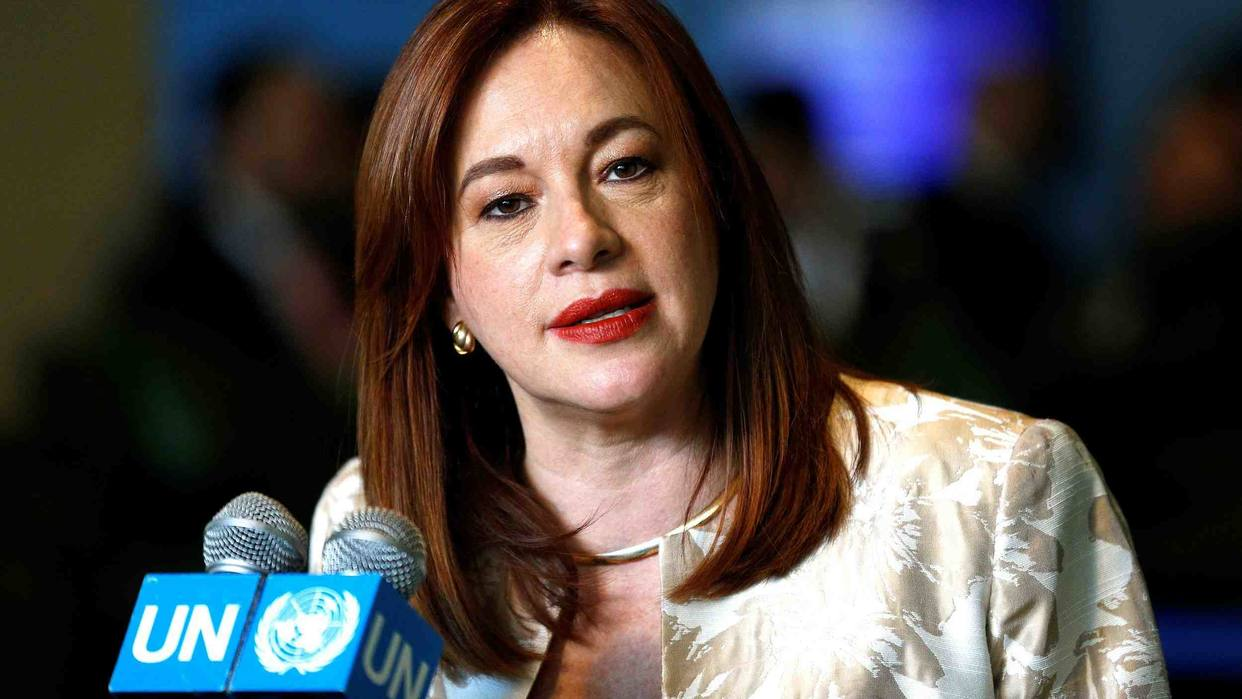
\includegraphics[width=300px]{202.jpg}%
\newline%
%
María Fernanda Espinosa, presidenta de la Asamblea General de Naciones Unidas,~aseguró que ha sido testigo de desarrollos positivos~de las~crisis en~Venezuela~y Nicaragua.%
\newline%
%
En el caso de~Venezuela, la diplomática ecuatoriana destacó la invitación del gobierno venezolano a la Alta Comisionada de la ONU para los Derechos Humanos, Michelle Bachelet, para que visite el país.%
\newline%
%
Mientras, en Nicaragua, apuntó al diálogo establecido entre las autoridades y la Secretaría General de Naciones Unidas, que consideró "muy prometedor".%
\newline%
%
"Creo que son desarrollos positivos en el sentido de volver a la calma y a la garantía de que en esos países se retome la normalidad y la población viva con toda la tranquilidad que merece", señaló Espinosa en una conferencia de prensa.%
\newline%
%
Espinosa aseguró que va a estar "muy atenta a cualquier desarrollo" en esos dos países y reiteró su llamamiento al "diálogo".%
\newline%
%
\end{document}